% !Tex root = main.tex


%sucasny stav riesenia problematiky dopisat ako sekciu ako sa ten problem riesi
% co riesime prepisat lepsie nas sposob
% 

\chapter{Opis problému}
% \chapter{Opis problému.}

V tejto kapitole formulujeme problém, ktorý riešime a hovoríme aj o súčasnom stav jeho riešenia. Spomíname viacero prístupov od autorov, ktoré tento problém riešia.

% TODO: mozno viac dodat, ze ake obmedzenia atd, ale to mozno neskor

%V časti Súčasný stav riešenej problematiky doma a v zahraničí autor uvádza dostupné informácie a poznatky týkajúce sa danej témy. Zdrojom pre spracovanie sú aktuálne publikované práce domácich a zahraničných autorov. Podiel tejto časti práce má tvoriť približne 30 % práce.
% optimalny plan nabijania asi nie






\section{Súčasný stav riešenej problematiky.}
\label{sucasny-stav}
Množstvo elektrických vozidiel (okrem dvojkolových a trojkolových) sa má podľa predikcií \cite{iea2023} zvýšiť od takmer 30 miliónov áut v roku 2022 po 240 miliónov áut roku 2030. V takom scénari by elektrické vozidlá tvorili viac ako $10\%$ zo všetkých cestných vozidiel.  \cite{iea2023} 
% Kapacity nabíjacích staníc by pri nabíjaní čoraz väčšieho množstva elektromobilov nemuseli stačiť. 



% adaptive
% Zvýši sa počet nielen súkromných elektrických aút, ale aj počet elektrických autobusov v mestskej hromadnej dopravne. \cite{iea2023} 
% cast pod tym je ok  cast nad tzm 

% elektromobil je vozidlo pohanane elektrickym motorom, zdroje: alza, ceska wiki a dalsia stranka

Veľa nabíjacích staníc dnes neriadí nabíjanie elektrických vozidiel, čo znamená, že nabíjačky nabíjajú elektrické vozidlá najväčším povoleným množstvom energie. Neriadené nabíjanie väčšieho množstva elektrických vozidiel už nebude použitelné, lebo neberie do úvahy obmedzenia infraštruktúry nabíjacej siete na energiu. \cite{lee2021acnsim} Pokroky v architektúre nabíjacej siete a v plánovaní nabíjania elektrických vozidiel umožnia nabíjanie väčšieho množstva  elektrických vozidiel za prijateľnú cenu a bez priveľkej záťaže na infraštruktúru nabíjacej siete. Súhrnne tieto pokroky voláme inteligentné (aj adaptívne) nabíjanie. \cite{lee2021adaptivephd,Lee2018LargeScaleAE}

% inteligentné nabíjanie alebo smart nabijanie

% neberie do uvahy ten jeden constraint
% TODO:roky a mnozstvo do matematickeho modu? 
Cieľom tejto práce je nájsť taký plán nabíjania elektrických vozidiel v nabíjacej stanici vďaka ktorému dokáže agregátor flexibility optimalizovať tok energie, zabezpečiť stabilné dodávky energie a minimalizovať náklady spotrebiteľov na energiu pri rešpektovaní obmedzení infraštruktúry nabíjacej siete. Správny plán nabíjania dokáže oddialiť náklady na vylepšenia infraštruktúry nabíjacej siete a pritom spĺňať stanovené vlastnosti. Algoritmy na nabíjanie elektrických vozidiel (plánovacie algoritmy) delíme do dvoch skupín online a offline. Offline algoritmy na plánovanie nabíjania elektrických vozidiel potrebujú všetky informácie o budúcich príchodoch elektrických vozidiel. Online algoritmy používajú informácie len o príchodoch elektrických vozidiel po aktuálny čas na plánovanie nabíjania  elektrických vozidiel. 

\begin{figure}[H]
    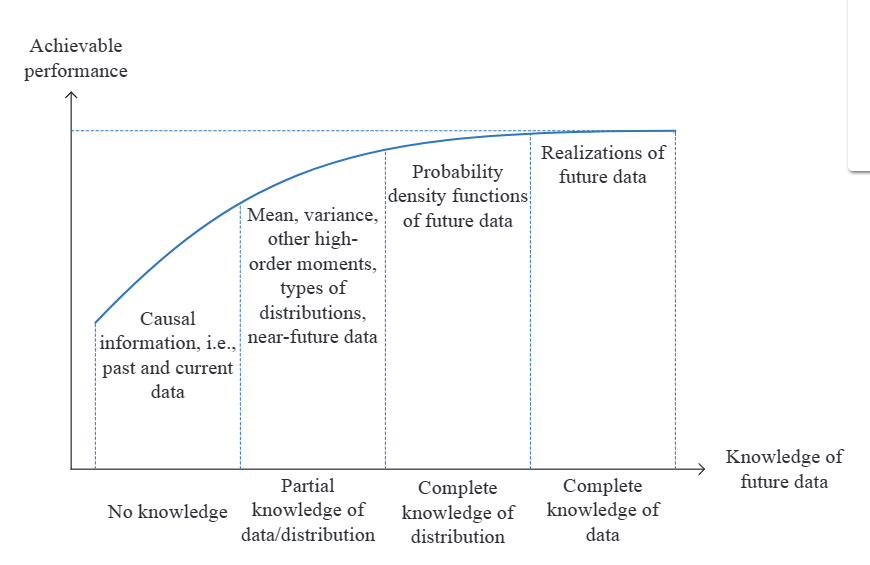
\includegraphics[width=\textwidth]{images/future_knowledge_cars.png}
    \centering
    \caption[Vplyv vedomostí o budúcich príchodov elektromobilov na výkonnosť plánovacieho algoritmu.]{Graf z článku \cite{Tang2016OnlineCS}, ktorý ilustruje vplyv vedomostí o budúcich príchodoch elektrických vozidiel na výkonnosť plánovacieho algoritmu.}.
    \label{architectureacnsim:obr2}
    \end{figure}



Bežné online plánovacie algoritmy (ako napríklad Earliest Deadline First, Least Laxity First) vieme použiť, aby sa infraštruktúra nabíjacej siete nepreťažovala, ale nedokážu vyprodukovať plán nabíjania elektrických vozidiel, ktorý napríklad minimalizuje náklady spotrebiteľov.  \cite{lee2021adaptivephd,chen2021smoothed} Výskumníci dokázali nájsť plán nabíjania s týmito vlastnostami vďaka trom prístupom: 


% Model Predictive Control (skrátene MPC), učenia posilňovaním a dynamického programovania.
% \begin{enumerate}
%     \item Model Predictive Control (skrátene MPC). Autori článkov \cite{mpcpredictive_uncertainty, Zhang2018RealTimeSC} používajú tento prístup..
%     \item Učenie posilňovaním. Tento prístup používajú v autori článkov \cite{rl_costmin_1}.
%     \item Dynamické programovanie. Týmto prístupom autori článku \cite{jakus2023optimal} riešia cieľ tejto práce.
% \end{enumerate}
% TODO najst dalsie clanky k DP
% Model Predictive Control (MPC), učenie posilňovaním alebo 

\begin{table}[H]
    \begin{tabular}{ll}
    Prístup                        & Článok \\
    Model Predictive Control (MPC) &      \cite{Lee2018LargeScaleAE}      \\
    Učenie posilňovaním            &   \cite{rl_costmin_1}        \\
    Dynamické programovanie        &   \cite{Zhang2018RealTimeSC}
    \end{tabular}
    \end{table}


    Autori článku \cite{Lee2018LargeScaleAE} implementujú online plánovací algoritmus Model Predictive Control, ktorý je schopný riešiť náš cieľ práce pomocou metód konvexnej optimalizácie. Plánovací algoritmus MPC popísaný v tomto článku sa odlišuje od ostatných MPC algoritmov tým, že uvažuje obmedzenie trojfázovej nevyváženej infraštruktúry nabíjacej siete a neideálne správanie batérie elektrického vozidla. Najpodstatnejší rozdiel je v tom, že je možné zadať viacero cieľov systémových operátorov v účelovej funkcií v MPC algoritme, ktoré rieši algoritmus MPC pomocou metód konvexnej optimalizácie. Porovnávanie výkonnosti algoritmov vykonávajú na trojfázovej nevyváženej infraštruktúre nabíjacej stanice Caltech ACN so vstupnými dátami z článku \cite{acndata}.
    % Pri porovnávaní plánovacieho algoritmu MPC s inými algoritmami používajú trojfázovú nevyváženú infraštruktúru nabíjacej stanice Caltech ACN. 
    
    % Algoritmus Model Predictive Control porovnávajú s algoritmom neriadeného nabíjania. Používajú pritom vstupné dáta z ACN [zdroj]
    % Na realistickej trojfázovej nevyváženej infraštruktúre Caltech ACN nabíjacej stanice 


    V \cite{Zhang2018RealTimeSC} autori implementujú dvojfázový aproximačný algoritmus dynamického programovania s cieľom dodať elektrickým vozidlám ich požadovanú energiu a minimalizovanť náklady za nabíjanie elektrických vozidiel na parkoviskách komerčných budov. Vstupné dáta o prichádzajúcich elektrických vozidlách modelujú na základe Poissonovej distribúcie. Na zistenie funčknosti ich algoritmu porovnali ceny nabíjania pri nabíjaní pomocou ich algoritmu s cenou nabíjania pomocou bežného aproximačného algoritmu. Zistili, že ich algoritmus v porovnaní s bežným aproximačným algoritmom dynamického programovania dosahuje v priemere o $2.5\%$ nižsiu cenu nabíjania elektrických vozidiel.
    % Na scénaroch s týmito vstupnými dátami porovnali náklady na nabíjanie energie ich algoritmu s bežným aproximačným algoritmom dynamického programovania.  

% V \cite{jakus2023optimal} autori implementujú program zmiešaného celočíselného programovania.




% ziadne rovnice v tejto sekcii okrem tej tabulky



% TODO: zmenit
% V poslednom desaťročí sa vedci snažili hľadať rôzne ďalšie algoritmy, ktoré by vedeli vyriešiť problém nabíjania elektromobilov pri zachovaní obmedzení infraštruktúry. \cite{iea2023} Potreby používateľov elektromobilov ako spotrebiteľov sú veľmi dôležité pri formulovaní optimalizačného problému, ktorý má tieto algoritmy riešiť.



% My sa venujeme optimalizačnému problému dodania najväčšieho množstva požadovanej energie elektromobilom pri zachovaní obmedzení infraštruktúry siete. Riešením tohoto problému vieme zabezpečiť to, že nabíjané elektromobily získajú čo najväčšie množstvo požadovanej energie. 


% acnsim clanok 


% Neriadené nabíjanie, ktoré dnes veľa nabíjacích staníc pre elektrické vozidlá využíva na nabíjanie ele sa už nebude môcť  



% ako problem riesia iny - pouzit priklady, ktore sme nepouzili, lebo je divne pisat o tom istom dvakrat

% \section{Súčasný stav riešenej problematiky}
% \section{Súčasný stav riešenej problematiky v reálnom živote.}


% Problematiku riešenia optimalizačného problému dodania najväčšieho množstva požadovanej energie elektromobilom pri zachovaní obmedzení infraštruktúry riešia v článkoch \cite{lee2021adaptivephd,Li_2021,chen2021smoothed}. 
% Na riešenie tohoto optimalizačného problému sa v súčasnosti využíva neriadené nabíjanie, spomína sa v \cite{lee2021acnsim}. Jednou z komplikácii pri takomto riešení optimalizačného problému je, že môže dôjsť k preťaženiu infraštruktúry nabíjacej siete. Nižšie spomíname, ako tento optimalizačný problém riešia v literatúre, a ako ho riešime my. \cite{lee2021acnsim}


% \section{Súčasný stav riešenej problematiky v literatúre.}

% V dostupnej literatúre je veľa zaujímavých algoritmov, ktoré sa však nedájú využiť priamo v praxi. Hlavným dôvodom prečo sa nedajú aplikovať je poďla \cite{lee2021adaptivephd} to, že výchádzajú z predpokladov, ktoré v praxi nefungujú alebo im chýba schopnosť splniť praktické obmedzenia a ciele. 
% % viac specifikovat prakticke obmedzenia a ciele

% V článku \cite{Li_2021} tento problém rieši hlavne systémový operátor. Systémový operátor vyrieši optimalizačný problém, a tým získa množstvo energie, ktorú pošle agregátorovi.  Agregátor pomocou plánovacieho algoritmu získa plán nabíjania elektromobilov a dodá energiu elektromobilom.



% My pri riešení tohoto optimalizačného problému využívame online plánovacie algoritmy s využitím balíka acnportal. Vstupom do online algoritmov sú elektromobily a ich parametre, ako napríklad čas ich príchodu, čas ich odchodu a ich požadovaná energia. Pomocou online plánovacích algoritmov získame poradie, v ktorom elektromobily nabíjame. Aby sme zistili množstvo energie, ktorú treba každému elektromobilu dodať, musíme vyriešiť spomínaný optimalizačný problém. Naším zámerom je riešiť optimalizačný problém osobitne pre každý elektromobil. Tento optimalizačný problém riešime metódou lineárneho vyhľadávania, metódy bisekcie, metódy dichotómie a pomocou kontrolných algoritmov (MPC). Riešením tohoto optimalizačného problému je optimálny plán nabíjania elektromobilov vzhľadom k dodanej energii.




% formulacia problemu/ ciel 
% vstup + (priklad)
% vystup + (priklad)
% obmedzenia


% There is a vast literature of algorithms for smart EV charging, which are outlined in
% [23] and [24].

% 23 link below
% https://www.researchgate.net/publication/290451911_Smart_Charging_for_Electric_Vehicles_A_Survey_From_the_Algorithmic_Perspective

% 24 link below
% https://www.researchgate.net/publication/286801210_A_Review_of_Charge_Scheduling_of_Electric_Vehicles_in_Smart_Grid


%  elektricke vozidlo = elektromobil > elektricke auto

% EV - either full electric source or also internal combustion engine

% preto je dobre aj zmenit elektromobil na elektricke vozidlo
% pridat tam aj indexovane parametre? zatial nie lebo mozno sa zide pouzivat aj ine velicy na indexovanie
% mozno pridat dalsie tabulky s dalsimi udajmi
V tabuľke nižšie popisujeme notáciu, ktorú používame v tejto práci. 
% dat left a right pred () zatvorky ak je tam tazsi matematicky vyraz
\begin{table}[H]
    \begin{center}
        \begin{tabular}{ c c }
         $V$ & Množina elektrických vozidiel. \\ 
         $V_{k}$ & Množina aktívnych (pripojených) elektrických vozidiel na nabíjacej stanici v čase $k$.  \\  
         $K$ & Množina časov $\left(K:= \{1, 2, \dots\}\right)$. \\
         $\delta$ & Dĺžka časového intervalu (jednotka: minúty). \\
         $a_{i}$ & Čas príchodu (pripojenia) elektrického vozidla $i$ \\  & normalizovaný na základe množiny časov $K$ ($a_{i} \in K$). \\  
         $d_{i}$ & Čas odchodu (odpojenia) elektrického vozidla $i$ \\  & normalizovaný na základe množiny časov $K$ ($d_{i} \in K$). \\  
         $e_{i}$ & Požadovaná energia elektrického vozidla $i$ (jednotka: kWh).  \\ 
         $e_{i}(k)$ & Zostávajúca požadovaná energia elektrického vozidla $i$ v čase $k$.  \\
         $d_{i}(k)$ & Zostávajúci čas nabíjania elektrického vozidla $i$ v čase $k$. \\
         $r_{i}(k)$ & Rýchlosť nabíjania elektrického vozidla $i$ v čase $k$ (jednotka: kWh).   \\ 
         $\overline{r}_{i} $ & Maximálna rýchlosť nabíjania elektrického vozidla $i$ (jednotka: kWh). \\
         $P(t)$ & Kapacita nabíjacej siete na energiu. \\
         $[x]^{+}$ & Projekcia $x$ do množiny reálnych nemínusových čísel $R^{+}$.  \\
         $[x]_{a}^{b}$ & Projekcia $x$ na interval $[a, b]$. 
    
         
        \end{tabular}
        \caption{Notácia.}
        \label{tab:notation}
        \end{center}
    \end{table}


% TODO zistit ci pri formulacii problemu tam pisu uvod do problemu alebo nie
\section{Formulácia problému.}
% optimálny nie lebo MPC offline je optimum a my hladame v online algoritmoch
% ciel problemu
% Riešime problém hľadania takého plánu nabíjania elektromobilov v nabíjacej stanici, ktorý zabezpečí stabilné dodávky energie elektromobilom a zníži náklady spotrebiteľov za nabitú energiu.



Model systému, v ktorom problém riešime, pozostáva z jednej nabíjacej stanice, ktorá obsluhuje množinu elektrických vozidiel $V$.
% , pričom jeden elektromobil z množiny $V$ označujeme $i$.
 Používame model systému s diskrétnym časom. V modeli systému s diskrétnym časom je čas $k \in K$ rozdelený do časových intervalov s rovnakými dĺžkami $\delta$. 
%  rovnako dlhých časových intervalov (dĺžku časových intervalov označujeme $\delta$). 
 Každé prichádajúce elektrické vozidlo $i \in V$ sa pripojí na nabíjačku na nabíjacej stanici v čase $a_i$ s požadovanou energiou $e_i$ a s časom odchodu $d_i$ a maximálnou rýchlosťou nabíjania batérie $\overline{r}_{i}$. Nabíjacia stanica obsluhuje v čase $k \in K$ všetky aktívne elektrické vozidlá $i \in V_{k}$ ($V_{k} \subseteq V$). Každé elektrické vozidlo reprezentujeme pomocou štvorice $(a_{i}, d_{i}, e_{i},\overline{r}_{i}) \in R^{4}$.   \cite{chen2021smoothed, Lee2018LargeScaleAE, Li_2021} Obmedzenia, ktoré dodržiavame počas nabíjania elektrických vozidiel sú:

%  pozriet ci aj oni tam pisu ze obmedzenia v systemovom modeli 
% Množinou $V_{k}$ označujeme všetký aktívne elektromobili (=elektromobily, ktorým ešte nebola dodaná požadovaná energia $e_{i}$ v čase $k$) v nabíjacej stanici v čase $k$ (platí, že $V_{k} \subseteq V$). 

% Stav elektromobilu $i$ v čase $k$ je štvorica hodnôt $(a_{i}, d_{i}, e_{i},\overline{r_{i}})$ 
% % $(e_{i}(k), \, d_{i}(k), \, \overline{r_{i}}(k))$,

% kde $e_{i}(k)$ je množstvo zostávajúcej požadovanej energie elektromobilu $i$ v čase $k$, $d_{i}(k)$ je zostávajúci čas do konca nabíjania elektromobilu $i$ v čase $k$ a $\overline{r_{i}}(k)$ je maximálna rýchlosť nabíjania elektromobilu $i$ v čase $k$. 



% Lepsie je uviest basic veci aby clovek nemusel citat dalsi clanok aby pochopil, ale na komplikovanejsie veci sa radsej odkazuj na dany clanok kde to bolo spomenute


% smoothed asi ciel prace dali do introduction


% Constraints

\renewcommand{\labelenumi}{\alph{enumi})}


% v adaptive maju maximalnu rychlost nabijania vztahujuca sa na cas
% v PPC nemaju 

% ak by sme mali online, tak nemusime definovat ak t < a_i, ale zatial pracuejeme s offline definicou


% how to align equations to left

% rethink indexing of time if u use the 


% elektromobil vymenit za elektricke vozidlo -> lepsie to znie


% oznacenie rovnic sa zide 
% subequations umoznuje ich pomenovavat napr (1a), ... (1d) bez toho je to (1),..(N)



\begin{subequations}
\begin{align}
    0 \leq r_{i}(k) \leq \overline{r}_{i}, & \qquad a_{i} \leq k < d_{i}, \; i  \in V \label{basic-constraints:subeq1}  \\
    r_{i}(k) = 0,  & \qquad   k \geq d_{i},\;  i \in V  \label{basic-constraints:subeq2} \\
    r_{i}(k) = 0, & \qquad k < a_{i},  \; i \in V \label{basic-constraints:subeq3} \\
    \sum_{k = a_{i}}^{d_{i} - 1} r_{i}(k) \delta \leq e_{i} & \qquad i \in V \label{basic-constraints:subeq4}\\
    f_{j}(r_{1}(k), \dots, r_{i}(k)) \leq R_{j}(k) &   \qquad j \in \hat{R} , \; i \in V \label{basic-constraints:subeq5}
\end{align}
\end{subequations}
% maximalna - je to slovenske slovo???
% elektromobil -> elektricke vozidlo treba zmenit kedze EV pouzivaju v publikaciach elektromobil = BEV v anglictine, EV = elektricke vozidlo = BEV + PHEV
Obmedzenie \eqref{basic-constraints:subeq1} zaručuje, že rýchlosť nabíjania $r_{i}(k)$ môže byť nanajvýš rovnaká ako maximálna rýchlosť nabíjania $\overline{r}_{i}$ pre elektrické vozidlo $i$ a čas $k$. Nabíjanie len aktívnych (pripojených) elektrických vozidiel v nabíjacej stanici zabezpečujú obmedzenia \eqref{basic-constraints:subeq2} a \eqref{basic-constraints:subeq3}. Nabíjanie elektrických vozidiel maximálne ich požadovanou energiou zabezpečuje obmedzenie \eqref{basic-constraints:subeq4}.  Obmezenie \eqref{basic-constraints:subeq5} používame na zabezpečenie množiny obmedzení $\hat{R}$ infraštruktúry nabíjacej siete. Funka $f_{j}$ je konvexná funkcia, ktorá mapuje nticu $(r_{1}(k), \dots, r_{N}(k))$ na agregovanú rýchlosť nabíjania $f_{j}(r_{1}(k), \dots, r_{N}(k))$ ($f_{j}: R_{+}^{N} \rightarrow R_{+}$). Obmedzením \eqref{basic-constraints:subeq5} zabezpečujeme, že agregovaná rýchlosť $f_{j}(r_{1}(k), \dots, r_{N}(k))$ nabíjania nepresahuje limit infraštruktúry $R_{j}(k)$ pre každé $j \in \hat{R} $. Obmedzenia infraštruktúry nabíjacej siete $j \in \hat{R}$ sú:






% vzdy skontrolovat ci hyperlinky funguju - v tomto pripade zjavne funguju po tento text




% uviest info ako funguje ta funkcia f ako to ma vplyv na obmedzenia 






% adaptive charging kniha ma prilis komplikovane zapisany posledny constraint, takze je lepsie cerpat z Large Scale ... 



% r_i(k) ma asi jednotku kWh nasvedcuje clanok smoothed least laxity 

% treba tie obmedzenia zmenit ak pouzijeme MPC s optimalizacnym horizontom, potom ten cas bude urceny pre optimalizacny horizont


% \begin{align*}
%     & a_{ijk} = 2 \\
%     &(because ||V_1-V_2|| = \max_{i \in [d]}|V^i_1 - V^i_2|)
%     \end{align*}





Obmedzenia systémového modelu, ktorý používame rozďeľujeme takto:
% mozno pridat ze prve obmedzenia su linearne a druhe SOC


% PPC mozeme pouzit len na jednofazove obmedzenia pre trojfazove by sa tazko robila odmena - navrh na vylepsenie
\begin{enumerate}
    \item Jednofázové obmedzenia infraštruktúry. Tieto obmedzenia infraštruktúry sa často používajú a sú vhodné len keď sú všetky nabíjačky jednofázové. V tejto práci pracujeme s jedným jednofázovým obmedzením:
    \begin{equation}
        \sum_{i \in V_{k}} r_{i}(k) \leq R,
    \end{equation}
    $\forall k \in K$. Bližší popis jednofázových obmedzení infraštruktúry je v článku \cite{Lee2018LargeScaleAE}.
    asi s nevyvazenymi trojfazovymi by to neslo
    \item Nevyvážené trojfázové obmedzenia infraštruktúry. Popis týchto obmedzení a aj ich odvodenia sa nachádzajú v článku \cite{Lee2018LargeScaleAE}.
\end{enumerate}
% Parametre systémového modelu, ktoré nastavujeme je počet a typ nabíjačiek a kapacita transformátora. Musíme si zvoliť aj ceny za nabíjanie (napríklad tarify). \cite{lee2021acnsim,Lee2018LargeScaleAE}.


% odkial pochadzaju vstupne data sa da dat aj do casti experimenty
% takisto vystupne data treba v casti experimenty specifikovat
% aj smoothed least laxity first to ma tak 

% Problém, ktorý riešime formulujeme takto:
% Hľadáme plán nabíjania elektromobilov v nabíjacej sieti, ktorý zabezpečí stabilné dodávky energie spotrebiteľom a zároveň minimalizuje náklady spotrebiteľov. 
% minimalizuje náklady spotrebiteľov na energiu 
% zabezpečí maximálne dodávky požadovanej energie. 
% vstup
% Vstupom algoritmu, ktorý tento problém rieši je zoznam aktívnych elektromobilov, kde je pre každý elektromobil určený jeho čas príchodu, čas odchodu a množstvo požadovanej energie. Aktívnym elektromobilom rozumieme taký elektromobil, ktorý je napojený na nabíjaciu stanicu a ešte nedostal svoju požadovanú energiu. 
% % V prípade online algoritmu, ktorý rieši tento problém zisťujeme plán nabíjania postupne pre každý časový krok.
% % vystup
% Výstupom algoritmu riešiaceho tento problém je slovník (plán nabíjania), ktorý mapuje nabíjačky na množstvá energie, ktoré poskytli po celú dobu nabíjania. Údaje o tom, aké nabíjačky nabíjali jednotlivé elektromobily vieme jednoducho zistiť cez triedu EV definujúcu elektromobily.


% Príklad výstupu:

% {
%     'CA-301': [32, 32, 32, 16, 16, ..., 8],
%     'CA-302': [8, 13, 13, 15, 6, ..., 0],
%     ...,
%     'CA-408': [24, 24, 24, 24, 0, ..., 0]
% }

% % inicializacia/nastavenia

% Plán nabíjania musí dodržiavať obmedzenia nabíjacej siete. Obmedzenia, ktoré nastavujeme pri riešení problému sú buď jednofázové alebo nevyvážené trojfázové. Bližší popis, z akých množín jednotlivé obmedzenia pozostávajú sa nachádza nižšie:
% \begin{enumerate}
%     \item Jednofázové. Jednofázové obmedzenia infraštruktúry sú množinou linearných obmedzení. 
%     \item Nevyvážené trojfázové. Nevyvážené trojfázové obmedzenia pozostávajú z množiny obmedzení kužeľa druhého rádu. Tento typ obmedzení má nabíjacia sieť Caltech ACN.
% \end{enumerate}
% % zistit ake ma JPL ci ma rovnake zda sa ze ano ale neviem potvrdit

% Ďalšie parametre nabíjacej siete, ktoré pri riešení problému nastavujeme sú nabíjačky (ich počet a typ), transformátor (jeho kapacita). Musíme si zvoliť aj tarify (ceny nabíjania v čase). Viac informácii o obmedzeniach, parametroch a tarifách  sa nachádza v článkoch \cite{lee2021acnsim,Lee2018LargeScaleAE}.


% % vysvetlit preco tento problem je optimalizacny problem



% % potrebujú na riešenie tohoto problému musia vyriešiť tento (optimalizačný) problém v každom časovom kroku:



% % SCS solver

% % otestovat v druhom experimente ci ich sLLF ma ine nabijanie nez LLF


% % 

% % ||c c||

% \begin{table}
% \begin{center}
%     \begin{tabular}{ | m{3em} | m{7cm}| } 
%      \hline
%      notácia & popis   \\ [0.5ex] 
%      \hline\hline
%      $V$ & množina všetkých elektromobilov  \\ 
%      \hline
%      $K$ & množina všetkých časových krokov v diskrétnom modeli \\ 
%      \hline
%      $k$ & časový krok v diskrétnom modeli \\ 
%      \hline

%      $\delta$ & dĺžka jedného časového kroku $k$  \\
%      \hline

%      $\mathcal{T}$ & optimalizačný horizont \\ 
%      \hline
%      $V_{k}$ & množina všetkých elektromobilov  \\ 
%      \hline
%      $R_{k}$ & množina riešení problému, ktoré spĺňajú všetky stanovené obmedzenia  \\ 
%      \hline



%      $r$ & optimalizačná premenná reprezentujúca plán nabíjania   \\
%         % pre optimalizačný horizont 
    
%     \hline
%     $r_{i}(t)$ & rýchlosť nabíjania pre elektromobil $i$ v čase $t$   \\   
%      \hline
%      $\overline{r}_{i}(t)$ & maximálna rýchlosť nabíjania pre elektromobil $i$ v čase $t$   \\
%      \hline
%     %  $\delta$ & 545   \\
%     %  \hline
%     %  5 & 88   \\ [1ex] 
%     %  \hline
%     \end{tabular}
%     \end{center}
% \end{table}
% % pozriet ci naozaj max z konvexnej 
%     Ide o optimalizačný problém lebo sa snažíme hľadať najlepšie riešenie z množiny možných riešení. Matematicky tento problém formulujeme takto:


% % ucenie posilnovanim
% % 
% % \begin{align}
% %     \overset{SCH}{\underset{r}{min}} \; U_{k}(r) \\
% %     U_{k}(r) = \sum_{t=1}^{k} c_{t} \cdot r_{t}
% % \end{align}


% % offline verzia:

% % \begin{align}
% %     \underset{u_{1},...,u_{T}}{min} C_{T} (u_{1}, \dots, u_{T}) \\ 
% %     \text{subject to  } \forall t=1,\dots,T: \\ 
% %     x_{t + 1} = f_{t}(x_{t}, u_{t}), \\
% %     x_{t} \in X_{t}, \\ 
% %     u_{t} \in U_{t} 
% % \end{align}

% % Môžeme tento problem prepisať na tento problém:
% % \begin{align}
% %     \underset{u \in U_{t}}{inf}   \sum (c_{t}(u_{t}) - log p^{*}(u_{t} | u_{t}))
% % \end{align}

% % V 








%     %  U_{k}(r) is not strictly concave function

%     % The sum of two concave functions is itself concave and so is the pointwise minimum of two concave functions, i.e. the set of concave functions on a given domain form a semifield.

%     % je to aj v smoothed laxity least clanku a aj v phd adaptive spomentuje ze je konkavna




% \begin{alignat}{2}
%     \label{eq:max_problem-general}
%     \overset{SCH}{\underset{r}{\max}} \; U_{k}(r) \\
%     \label{eq:utility-function-general}
%     U_{k}(r) = \sum_{i \in V,
%                     t \in \mathcal{T}}r_{i}(t) \\
%     \text{subject to:} \notag \\
%     \label{eq:first-linear-constraint}
%     0 ≤ r_{i}(t) ≤ \overline{r}_{i}(t)  && \qquad  \qquad  t < d_{i}, i ∈ V \\
%     \label{eq:second-linear-constraint}
%     r_{i}(t) = 0 && t ≥ d_{i}, i ∈ V \\
%     \label{eq:third-linear-constraint}
%     \sum_{t = a_{i}}^{d_{i} - 1} r_{i}(t) \delta ≤ e_{i} && i ∈ V \\
%     \label{eq:network-constraints}
%     f_{j}(r_{1}(t), \dots, r_{N}(t) ) ≤ R_{j}(t) && t ∈ T, j ∈ \hat{R}
%     % r \in R_{k}
% \end{alignat}
% Množina aktívnych elektromobilov $V_{k}$ definuje optimalizačnú premennú $r := (r_{i}(1), \dots, r_{i}(T))$ pre optimalizačný horizon $\mathcal{T} = \{1,\dots,T\}$.
% Nerovnica \ref{eq:first-linear-constraint} popisuje, že rýchlosť nabíjania $ r_{i}(t)$ musí byť v rozmedzí od 0 po maximálnu rýchlosť nabíjania.
% Rovnica \ref{eq:second-linear-constraint} popisuje, že rýchlosť nabíjania po odchode elektromobilu z nabíjacej stanice musí byť $0$. 

% Nerovnosť \ref{eq:third-linear-constraint} zabezpečuje, že elektromobilu dodáme nanajvýš toľko energie, koľko je požadovanej energie.
% % Nerovnosť \ref{eq:network-constraints} popisuje obmedzenia siete.

% Nakoniec nerovnosť \ref{eq:network-constraints} zabezpečuje fungovanie obmedzení infraštruktúry nabíjacej siete. Množina obmedzení infraštruktúry siete je $\hat{R}$. To znamená, že premenná $j$ je jedno obmedzenie z množiny $\hat{R}$. Pre každé obmedzenie $j$, $R_{j}(t)$ je kapacita nabíjacej siete pre čas $t$. Funkcia $f$ je konvexná funkcia ktorá mapuje $\forall i r_{i}(t) \rightarrow r(t)$, kde $r(t)$ je agregovaná hodnota nabíjania v čase $t$. 



% % Účelovú funkciu $U_{k}(r)$ definujeme takto:
% % $U_{k}(r) = \sum_{i \in V, 
% %                 }^{}$



% % vysvetlit co je mnozina R_k
% % vysvetlit jednotlive obmedzenia pod subject to 
% % vysvetlit co je f_j

% % co to je vztah kuzela druheho radu a konvexny problem

% Tento problém, ktorý riešime je kovexný problém spomína sa v (). Konkrétne ide o problém špeciálnej triedy konvexných problémov nazývajúcu sa kužeľ druhého rádu, lebo naša účelová funkcia, ktorú maximalizujeme je lineárna funkcia a obmedzenia sú lineárne a aj kužeľa druhého rádu. (uviest zdroj ...) V prípade, keby sme použili jednofázové obmedzenia siete, tak by sme pracovali s problémom lineárneho programovania (všetky obmedzenia a účelová funkcia sú lineárne).



% % tu ako my ho riesime

% % ake algoritmy pouzivame na tento problem
% Algoritmy, ktoré riešia tento problém sa nazývajú optimalizačné algoritmy. My spočiatku používame na riešenie tohoto problému optimalizačné metódy (metóda bisekcie, metóda lineárneho vyhľadávania, metóda zlatého rezu) v algoritmoch založené na triedení (LLF, EDF). Optimalizujeme plán nabíjania spočiatku pre jeden krok dopredu($\mathcal{T} = {1}$). Následne používame algoritmus PPC, ktorý rieši tento problém nazývajúci sa , 

% ujasnit co presne riesi, lebo to co riesi PPC je trochu ina rovnica 


% použitím MPC s $\mathcal{T} = {1, \dots, T}$. Online algoritmy riešia stanovený problém v každom časovom kroku $k$. 



% https://www.solver.com/conic-optimization#Second%20Order%20Cone%20Programming%20(SOCP)

% upravit zdroj zachary leeho diplomovky



% One of the most challenging parts of scheduling charging in a real system is that
% the algorithm does not know what the future holds. As new EVs arrive, or when
% users need to change their input parameters, the algorithm must adapt its schedule
% accordingly. ASA also incorporates many realistic constraints such as unbalanced
% three-phase infrastructure, control signal quantization, and battery management
% system behavior.


% 30,32

% 33,34

% 36

% 28,62
% 68

% 15 predict user behavior

% realistic environment for experiments

% 33- statistical model to MPC, with minor modifications 
% there was no algorithm in literature that satisfied adaptive 

% they dont consider other ev charging alg because they are not realistic -> to work with discrete pilot signals and
% unbalanced three phase infrastructure

% smart charging algorithms 24, 25





% To give us Property 7, we propose an algorithm called
% ramp-down to reclaim idle capacity from EVs that are not using their full allocation.
% The most common reason for this is the vehicle’s acceptance rate decreasing as the
% battery fills up, as we saw in Fig. 4.3.

% Whenever an event
% occurs or the time since the last charging schedule update exceeds a threshold (for
% example, 5 min), we compute a new charging schedule.

% \qquad
% Veľa riešení tohoto problému používa algoritmy založené na triedení a algoritmy na zdielanie procesov. Iné prístupy používajú učenie posilovaním, dynamické programovanie a model predictive control. Algoritmy založené na triedení najprv utrieda elektromobily podľa nejakého kritéria. 

% Každému elektromobilu je potom pridelené maximálne množstvo energie, ktoré sa vypočíta (pre optimalizačný horizont $T = {1}$) pomocou metódy bijekcie, ktorá maximalizuje jednotlivé komponenty siete $u_{k}^{v}(r)$, ktoré tvoria váhovaný súčet $U_{k}(r)$:
% \[
% U_{k}(r) := \sum_{v=1}^{V} a_{k}^{v} u_{k}^{v}(r),
% \]
% kde $a_{k}^{v} > 0, k \in K, v \in V$ sú časovo závislé váhy, ktoré priraďuju prioritu jednotlivým komponentom nabíjacej siete. 


% % účelová funkcia $u_{k}^{v}(r)$ má rovnaký tvar ako 6. rovnica v článku 
% Problém maximalizovania účelovej funkcie $u_{k}^{v}(r)$ definujeme takto:



% \begin{alignat}{2}
%     \label{eq:max_problem-specific}
%     \underset{r_{i}(t)}{\max} \; u_{k}^{v}(r) \\
%     \label{eq:utility-function-specific}
%     u_{k}^{v}(r) = r_{i}(t) \\
%     \text{subject to:} \notag \\
%     \label{eq:first-linear-constraint-specific}
%     0 ≤ r_{i}(t) ≤ \overline{r}_{i}(t)  && \qquad  \qquad  t < d_{i}, i ∈ V \\
%     \label{eq:second-linear-constraint-specific}
%     r_{i}(t) = 0 && t ≥ d_{i}, i ∈ V \\
%     \label{eq:third-linear-constraint-specific}
%     \sum_{t = a_{i}}^{d_{i} - 1} r_{i}(t) \delta ≤ e_{i} && i ∈ V \\
%     \label{eq:network-constraints-specific}
%     f_{j}(r_{1}(t), \dots, r_{N}(t) ) ≤ R_{j}(t) && t ∈ T, j ∈ \hat{R}
%     % r \in R_{k}
% \end{alignat}{2}



% toto este upravit -
% \begin{alignat}{2}
%     \label{eq:max_problem-general}
%     {\underset{r}{\max} \; u_{k}^{v}(r) \\
%     \label{eq:utility-function-general}
%     U_{k}(r) = \sum_{i \in V,
%                     t \in \mathcal{T}}r_{i}(t) \\
%     \text{subject to:} \notag \\
%     \label{eq:first-linear-constraint}
%     0 ≤ r_{i}(t) ≤ \overline{r}_{i}(t)  && \qquad  \qquad  t < d_{i}, i ∈ V \\
%     \label{eq:second-linear-constraint}
%     r_{i}(t) = 0 && t ≥ d_{i}, i ∈ V \\
%     \label{eq:third-linear-constraint}
%     \sum_{t = a_{i}}^{d_{i} - 1} r_{i}(t) \delta ≤ e_{i} && i ∈ V \\
%     \label{eq:network-constraints}
%     f_{j}(r_{1}(t), \dots, r_{N}(t) ) ≤ R_{j}(t) && t ∈ T, j ∈ \hat{R}
% \end{alignat}{2}







% Tento prístup je dobrý preto, že oproti bežným algoritmom založených na triedení (ktoré používajú lineárne vyhľadávanie na zistenie rýchlosti nabíjania ) používa pokročilejšie metódy (metóda bisekcie, metóda zlatého rezu) na zistenie rýchlosti nabíjania.
% najst zdroj

% $\mathcal{T}$







% Potom, algoritmy založené na triedení maximalizujú pre každý elektromobil i $u_{k}^{i}(r)$. Maximalizovaním $u_{k}^{i}(r)$ maximalizujeme účelovú funkciu $U_{k}(r)$


% Problém, ktorému sa venujeme je optimalizačným problémom, lebo hľadáme taký plán nabíjania, ktorý maximalizuje účelovú funkciu. 

% % zarovnat tu pravu cast nejako

% Formálnejšie definujeme tento optimalizačný problém takto:

% obidva pristupy riesia ten isty problem len inym sposobom

% $\overset{above}{main}$
% $\underset{\underset{r}{\max}}{SCH}$

% \begin{alignat}{2}
%     &\text{left side} &&= \text{right side} \\
%     &\text{left side that is longer} &&= \text{right side} \\
%     &\text{short} &&= \text{longer on the right side}
% \end{alignat}


%  max r(i)
% napisat R so striezkou neviem ako to spravit
% \ref{eq:einstein}

% sa snažíme maximalizovať množstvo dodanej energie elektromobilom. 












%  elektromobilom v nabíjacej sieti.








% Riešenie tohoto optimalizačného problému v článku+
% pozriet ako toxin li v tom jeho clanku spominal podobne riesenia


%first sentences of the thesis strong and clear - to get interest of the reader
\chapter{Cieľ práce}

Cieľ práce je navrhnúť a overiť model práce agregátora flexibility pre zvolený typ prosumerov. V našom prípade považujeme vlastníkov elektrických vozidiel za prosumerov. Model práce agregátora flexibility je v našom prípade tvorba plánu nabíjania elektrických vozidiel pomocou plánovacích algoritmov. Plán nabíjania má spĺňať požadované vlastnosti:


% co su presne stabilne dodavky? ze nemoze byt velke oscilacie v nabijani???
\begin{enumerate}
    \item optimalizuje tok energie. V našom prípade optimalizujeme tok energie tak, aby sme dodali elektrickým vozidlám najväčšie množstvo ich požadovanej energie.
    \item zabezpečuje stabilné dodávky energie. To znamená, že plán nabíjania poskytuje elektrickým vozidlám bez prerušení a bez významných výkyvov v rýchlosti nabíjania.
    \item minimalizuje náklady spotrebiteľov na nabitú energiu. 
    \item rešpektuje obmedzenia \eqref{basic-constraints:subeq1}, \eqref{basic-constraints:subeq2}, \eqref{basic-constraints:subeq3}, \eqref{basic-constraints:subeq4}, \eqref{basic-constraints:subeq5},  počas nabíjania elektrických vozidiel.
\end{enumerate}

% TODO:pridat nieco do ciela prace? zatial nic

% Vstupom do plánovacich algoritmov, ktoré vyprodukujú plán nabíjania s požadovanými vlastnosťami 

% Presnejší popis cieľa práce sa nachádza v kapitole 


% To znamená, že musíme popísať ako agregátor flexibility dodáva energiu elektromobilom. Energiu agregátor flexbility bude dodávať elektromobilom na základe plánovacieho algoritmu, ktorý rieši optimalizačný problém [odkaz].  
% Vyriešime optimalizačný problém dodania najväčšieho množstva energie elektromobilom pri zachovaní obmedzení infraštruktúry.
%  Využívame pri riešení optimalizačného problému online plánovacie algoritmy (kontrolné alebo triediace), pričom vychádzame zo základných tried v balíku acn portal, ktoré definujú obmedzenia nabíjacej siete a zjednodušujú prácu s novo implementovanými algoritmami.
 
%  Vstupom algoritmu, ktorý rieši tento optimalizačný problém sú údaje o príchodoch elektromobilov do nabíjacej siete Caltech. Výstupom tohoto algoritmu je celkový pomer dodanej požadovanej energie elektromobilom a celkové cena dodanej energie elektromobilom atď. Overíme si navrhnutý model agregátora flexibility na verejne dostupných vstupných dátach z Caltech nabíjacej siete.  








% \section{Činnosti agregátora flexibility}


\section{Úlohy agregátora flexibility}


% V súčastnosti pozorujeme pokrok v oblasti distribuovania obnoviteľnej energie. 
% % S čoraz vyšším dopytom po energii sa 
% Výskumníci sa začali zaoberať výskumnou otázkou: Ako môžu spotrebitelia dodávať energiu a zároveň ju prijímať? Výskumníci našli riešenie tejto výskumnej otázky a popísali, čo treba na riešenie tejto výskumnej otázky:
% \begin{enumerate}
%     \item Zmeniť jednosmernú sieť, kde veľké firmy dodávajú energiu spotrebiteľom, na obojsmernú sieť, kde spotrebitelia dodávajú a zároveň prijímajú energiu (skrátene takých spotrebiteľov nazývame prosumeri).
%     \item Zaviesť novú kategóriu hráčov na trhu s energetikou. Túto novú kategóriu hráčov nazývame agregátori. 
% \end{enumerate}
% % . Výskumníci zaviedli novú kategóriu hráčov na trhu s energetikou. Túto novú kategóriu hráčov nazývame agregátori. 


Agregátor je prostredníkom medzi prosumermi a trhom s elektrinou, tým že združuje flexibilitu od prosumerov, a následne flexibilitu predáva (ako jedna entita) na trhoch s elektrinou. Prosumeri sú odmeňovaní za poskytovanie flexibility agregátorovi. V našom modeli predpokladáme, že prosumeri nie sú odmeňovaní za poskytovanie elektrickej energie agregátorovi.

% ako su odmenovani? a ako to funguje v nasom pripade
% ako moze predavat flexibilitu? nerozumiem


Rola agregátora zatiaľ nie je presne definovaná. Rola agrégatora môže byť určená tretou stranou alebo môže byť určená už učinkujúcim hráčom na trhu s elektrinou, ktorý má napríklad záujem použiť agregátor na doplňujúce veci.
%doplnujuce veci - vysvetlit

Nezávislý agregátor môže poskytovať jednu službu alebo viac služieb. Medzi služby agregátora patria agregovanie flexibility, dodávky energie spotrebiteľom a vyváženie dopytu a ponuky na trhoch s elektrinou. \cite{Granado2023}

% spomenut ako to funguje v nasom pripade


% Systémy v elektrickej sieti môžu mat jeden centrálny agregátor alebo viac agregátorov.






% Prosumeri poskytujú agregátorovi svoju flexibilitu. 




% Agregátor má viacero úloh, ktoré rieši. Agregátor združuje elektrickú energiu od prosumerov. Agregátor pozoruje cenu energie na trhoch. Ak je cena energie veľmi vysoká, tak agregátor poskytuje spotrebiteľom menej energie. Naopak, keď je cena energie nízka, tak agregátor poskytuje spotrebiteľom viac energie.


% optional link

% https://en.energinet.dk/Electricity/Green-electricity/Demand-side-response/What-is-an-aggregator/

% nedat toto tam lebo toto predpoklada obojsmernu siet
% \begin{figure}[H]
%     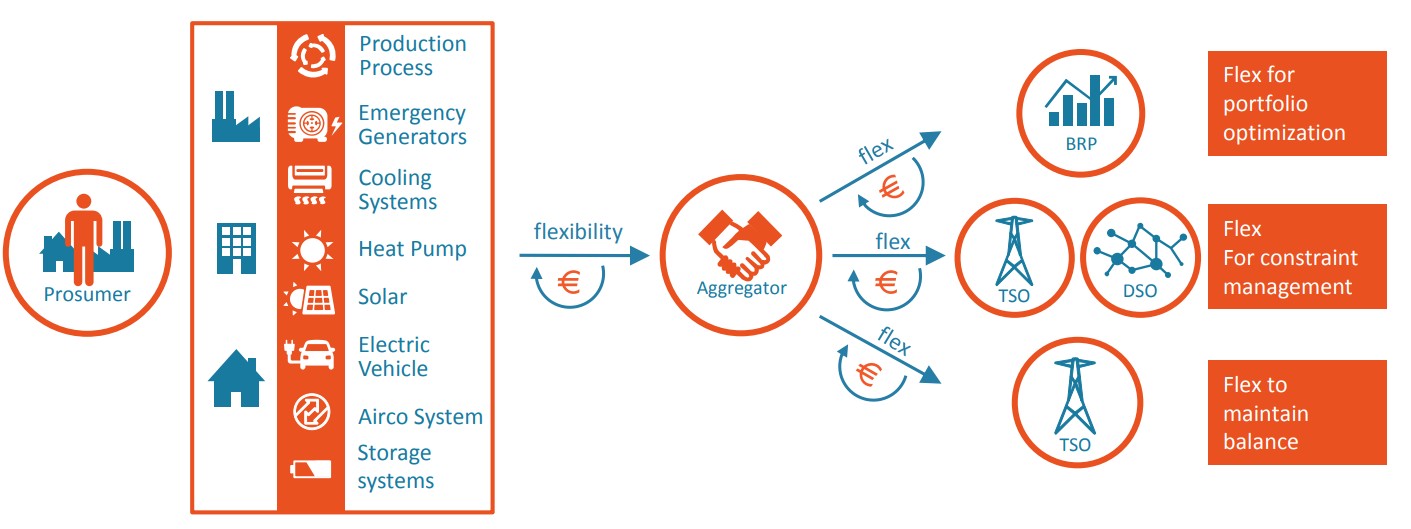
\includegraphics[width=\textwidth]{images/prosumers_aggregator.png}
%     \centering
%     \caption[Funkcie agregátora flexibility]{Distribúcia flexibility medzi prosumermi, agregátorom a trhom s elektrinou. Zdroj obrázka je \cite{usef2018}.}
%     % \label{onlinealg:obrnotyet}
%     \end{figure}

\begin{figure}[H]
    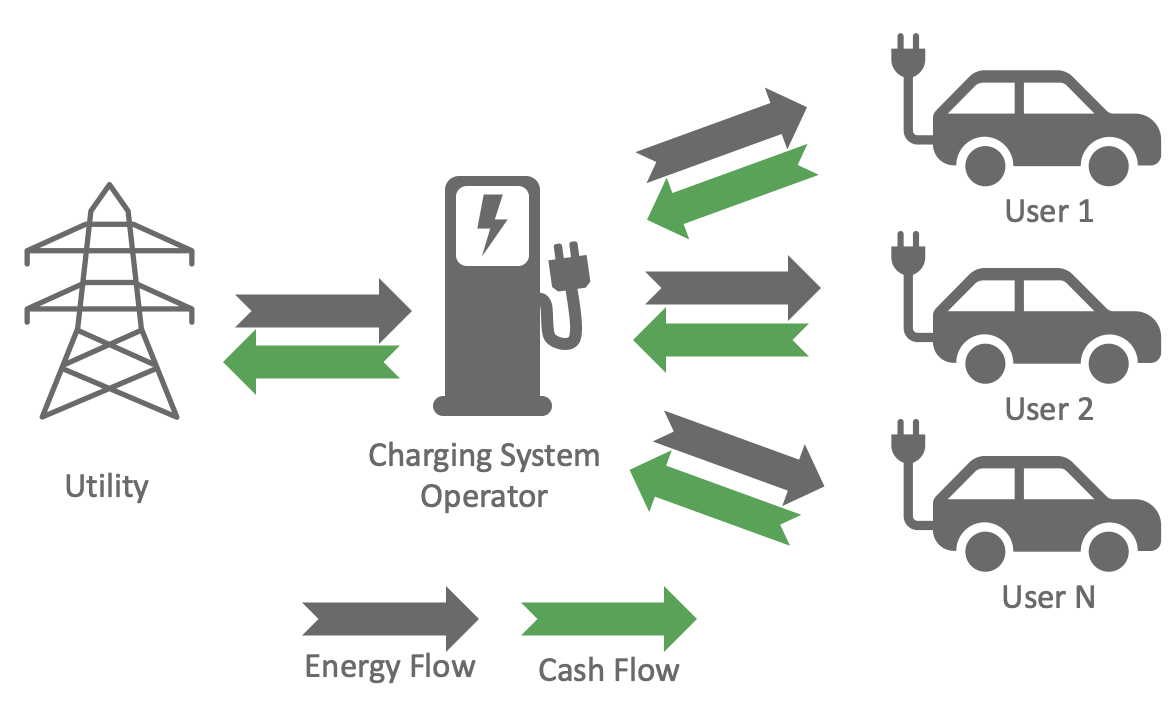
\includegraphics[width=\textwidth]{images/energy_flow_costs.png}
    \centering
    \caption[Systém toku energie a ziskov.]{Systéme toku energie a aj zisky za energiu. Agregátor (Charging System Operator) kupuje energiu od systémového operátora (utility). Agregátor sa musí rozhodovať: 1. koľko energie od systémového operátora kúpi 2. na rýchlosti nabíjania elektrických vozidiel  3. na distribúcii nákladov za energiu medzi spotrebitľmi elektrických vozidiel. Zdroj obrázka je: \cite{websitpricecharging2023}.}
    \label{architectureacnsim:obr2}
    \end{figure}

% overit ze taketo nazvy aggregator = charging system operator a utility= system operator sedia


% \UNFIN
% image source https://www.usef.energy/app/uploads/2016/12/USEF_IndependentAggregator.pdf

% \cite{KUBLI2021110908}

% \chapter{Východiská}
% \label{kapitola:vychodiska}
% V tejto kapitole popisujeme technologické a teoretické východiská, ktoré využívame v implementácii. Technologické východiská tvoria najmä Balíke, ktoré implementujú existujúce riešenia. Teoretické východiská zostávajú z veľkej časti podobné ako pri existujúcich riešeniach, aby sme vedeli následne efektívne porovnať našu implementáciu s existujúcimi riešeniami.


% \subsubsection*{Parametre spotrebiteľa.} 
% % \subsubsection*{Parametre spotrebiteľa} 

% Každému spotrebiteľovi $j = 1, \ldots, N$ je pridelená štvorica dát \\ $(a(j), d(j),  e(j), r(j)) \in R^{4}$. Parameter $a(j)$ znamená čas príchodu a parameter $d(j)$ je čas odchodu. Obe premenné sa normalizujú. Parameter $e(j)$ označuje množstvo požadovanej energie v jednotkách kWh a $r(j)$ je maximálne množstvo nabíjacej energie.

% \subsubsection*{Rozhodnutie agregátora.}
% % \subsubsection*{Rozhodnutie agregátora}
% Rozhodnutie agregátora v čase $t$ pre všetkých spotrebiteľov označujeme $s_{t}$. Premenná $s_{t}$ obsahuje pridelenie energie pre každého spotrebiteľa v čase $t$ na základe nejakého trediaceho algoritmu. Nech $\pi_{t}$ je použitý triediaci algoritmus (napr. Least Laxity First, Early Deadline First) v čase $t$. Potom premennú $s_{t}$ vypočítame takto:
% \begin{equation}
%     s_{t} = \pi_{t}(u_{t}),
% \end{equation}
% kde $u_{t} \in U$ je úroveň výkonu agregátnej rozvodne v čase $t$. 

% \subsubsection*{Stav agregátora.}
% % \subsubsection*{Stav agregátora}
% Stav agregátora v čase $t$ označujeme $x_{t}$. Hodnotu premennej $x_{t}$ zistíme takto:
% \begin{equation}
%     x_{t} = \{(d_{t}(j), e_{t}(j):a(j) < t < d(j)), j = 1, \ldots, N\},
% \end{equation}
% kde $e_{t}(j)$ je zostávajúca požadovaná energia a $d_{t}(j)$ je  zostávajúci čas na nabíjanie v čase $t$.

% \subsubsection*{Prechodové funkcie.}
% Každé rozhodnutie $s_{t}(j) \in R$ agregátora v čase $t$ pre spotrebiteľa $j$ zmení stav agregátora. Keď sa zmena aplikuje na všetkých spotrebiteľov stav agregátora sa zmení z $x_{t}$ na $x_{t + 1}$. Aplikujeme dve prechodové funkcie na $e_{t}(j)$ a na $d_{t}(j)$ takto:

% \begin{gather}
%     e_{t}(j) = e_{t - 1}(j) - s_{t}(j), \\ 
%     d_{t}(j) = d_{t - 1}(j) - \Delta,
% \end{gather}
% kde časový interval $\Delta$ je 12 minút. Predpokladáme, že nenastane žiadna strata energie. Tým dostaneme nový stav: 
% \begin{gather}
% x_{t + 1} = f(x_{t} \in X_{t}).
% \end{gather}  








% \subsubsection*{Podmienky pre rozhodnutie agregátora.}
% Podmienky, ktoré by mali byť rozhodnutím agregátora splnené sú:
% \begin{gather}
%     s_{t}(j) = 0, \text{ ak $t < a(j)$ alebo $t > d(j)$}, j = 1, \ldots N, \label{tv:pra:1} \\
%     \sum_{j = 1}^{N} s_{t}(j) = u_{t}, j = 1, \ldots N, \label{tv:pra:3} \\
%     \sum_{t = 1}^{T} s_{t}(j) = e(j), t = 1, \ldots T, \label{tv:pra:4}\\
%     0 \leq s_{t}(j) \leq r(j),t = 1, \ldots, T \label{tv:pra:5}.
% \end{gather}
% Obe podmienky~\ref{tv:pra:1} a~\ref{tv:pra:5} vždy platia. Dalšie uvedené podmienky nemusia nutne platiť.





% % \subsubsection{Maximum flexibility feedback.}
% % \subsubsection*{Maximálna odozva flexilibity.}
% % Nech $(p_{1}^{*}, \ldots, p_{n}^{*})$ je unikátne riešenie. Potom maximálnu odozvu entropie označujeme $p_{t}* = \psi_{t}(u_{t})$.

% % "Equation \ref{eq:quadratic} shows a quadratic function."




% % Operator vie naklady $(c_{1}, \dots, c_{n})$ a odozvu, ale nevie buduce naklady $(c_{i+1}, \dots, c_{T})$ a odozvu $(p_{i+1}, \dots, p_{T})$.


% % \subsubsection{Algoritmus hlbokeho ucenia}
% % \begin{equation}
% %     j(\psi) = \sum_{t = 1}^{T}E [r(x_{t},p_{t}) + aH(\psi(x_{t}))]. \label{eq:Jahu}
% % \end{equation}

% % MSE 
% % \begin{equation}
% % MSE = \frac{\sum_{k = 1}^{L} \sum_{k = 1}^{T} |\sum_{j = 1}^{N} s_{t}^{(k)}(j)  - u_{t}^{k}|^{2}}{L \cdot T \cdot \Omega}. \label{eq:MSE}
% % \end{equation}

% \subsubsection{MPE.} Chyba mean percentage error, v skratke MPE je pomer nedodanej energie k dodanej energii (porušenie podmienky \ref{tv:pra:4}). Počíta sa vzorcom:
% \begin{equation}
% MPE = 1 - \sum_{k = 1}^{L} \sum_{t = 1}^{T} \sum_{j = 1}^{N} \frac{s_{t}(j)}{\sum_{j = 1}^{N}e_{j}},  \label{eq:MPE}
% \end{equation}
% kde MPE nadobúda hodnoty z intervalu $[0, 1]$.



